\documentclass[12pt]{article}
\usepackage[none]{hyphenat}
\usepackage{fancyhdr}
\usepackage[english]{babel}
\usepackage{amsmath}
\usepackage{mathtools}
\usepackage{amsfonts}
\usepackage{amssymb}
\usepackage{graphicx}
\usepackage{hyperref}
\usepackage{titlesec}
\usepackage{graphicx,array}
\usepackage{geometry}
\usepackage{float}
\usepackage{textcomp}
\geometry{
 left=20mm,
 right=20mm,
 top = 20mm,
 bottom = 20mm,
 }
\newcolumntype{C}[1]{>{\centering\let\newline\\\arraybackslash\hspace{0pt}}m{#1}}
\newcolumntype{L}[1]{>{\raggedright\let\newline\\\arraybackslash\hspace{0pt}}m{#1}}

\setcounter{secnumdepth}{4}

\begin{document}
\begin{titlepage}
	\begin{center}
		\begin{figure}
			\centering
			
\includegraphics[height=54mm,width=55mm]{iitpkd.jpg}
		\end{figure}
			\Huge{CS4801: PRINCIPLES OF MACHINE LEARNING 2018}\\ \vspace{.5in}
			\huge{\textbf{Mini Project Report}}\\ \vspace{0.5in}
    \textbf{\Huge{Human Activity detection using Smartphones Data Set }}\\ \vspace{.5in}
    \huge{Project under - Dr. Sahely Bhadra}
    \end{center}
    \vfill
                \begin{large}\begin{center}Nikhil Kumar Yadav\\
		\vspace{15pt}
        Indian Institute of Technology, Palakkad\\
        Computer Science And Engineering Department\\
        Oct 29,2018\end{center}\end{large}
		
             
\end{titlepage}
\newpage
\section{Data Set Description}
This data set contains information obtained from 30 volunteers, within age bracket of 19-48 years, performing day to day activites like walking, walking upstairs,walking downstairs, sitting, standing and laying. The data is collected from the sensors of Samsung Galaxy S II mounted on the waists of the volunteers. The activites were manually labeled by watching videos of volunteers doing these tasks.

The sensor signals (accelerometer and gyroscope) were pre-processed by applying noise filters and then sampled in fixed-width sliding windows of 2.56 sec and 50$\%$ overlap (128 readings/window). The sensor acceleration signal, which has gravitational and body motion components, was separated using a Butterworth low-pass filter into body acceleration and gravity. The gravitational force is assumed to have only low frequency components, therefore a filter with 0.3 Hz cutoff frequency was used. From each window, a vector of features was obtained by calculating variables from the time and frequency domain.

The features selected for this database come from the accelerometer and gyroscope 3-axial raw signals tAcc-XYZ and tGyro-XYZ. These time domain signals (prefix 't' to denote time) were captured at a constant rate of 50 Hz. Then they were filtered using a median filter and a 3rd order low pass Butterworth filter with a corner frequency of 20 Hz to remove noise. Similarly, the acceleration signal was then separated into body and gravity acceleration signals (tBodyAcc-XYZ and tGravityAcc-XYZ) using another low pass Butterworth filter with a corner frequency of 0.3 Hz. 

Subsequently, the body linear acceleration and angular velocity were derived in time to obtain Jerk signals (tBodyAccJerk-XYZ and tBodyGyroJerk-XYZ). Also the magnitude of these 3-D signals were calculated using the Euclidean norm (tBodyAccMag, tGravityAccMag, tBodyAccJerkMag, tBodyGyroMag, tBodyGyroJerkMag). 

Finally a Fast Fourier Transform (FFT) was applied to some of these signals producing \\fBodyAcc-XYZ, fBodyAccJerk-XYZ, fBodyGyro-XYZ, fBodyAccJerkMag, fBodyGyroMag,\\ fBodyGyroJerkMag.

Then signals were then used to calculate their mean, std, meadian absolute deviation, max, min, signal magnitude area, energy, interquartile range, entropy, autorregresion coefficients, correlation, skewness, angle etc

This data set was pre-divided into training and test sets with traning set containing 7352 samples and test set containing 2947 samples.
\newpage
\section{Analytics}
Fig\ref{fig:dis} shows that data points are somewhat equally distributed.
\begin{figure}[H]
\centering
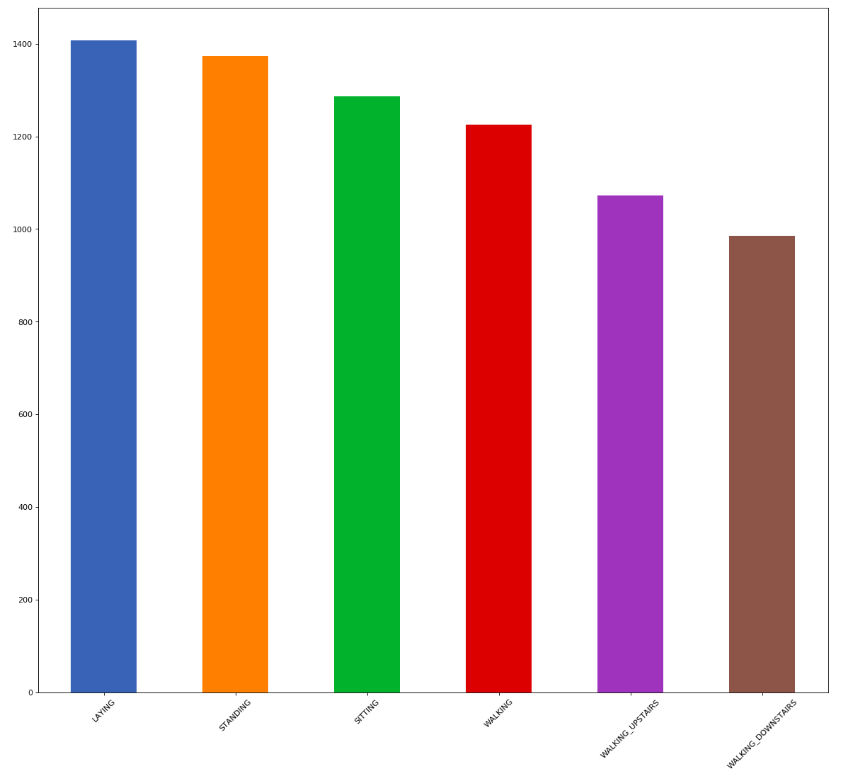
\includegraphics[scale=0.17]{dis.png}
\caption{Distribution of class labels}
\label{fig:dis}
\end{figure}\noindent
I am using t-SNE to visualize the data points. t-Distributed Stochastic Neighbor Embedding is a non-linear dimensionality reduction algorithm used for exploring high-dimensional data. It's outputs provide better results than PCA and other linear dimensionality reduction models. This is because a linear method such as classical scaling is not good at modeling curved manifolds. It focuses on preserving the distances between widely separated data points rather than on preserving the distances between nearby data points. The algorithm computes pairwise conditional probabilities and tries to minimize the sum of the difference of the probabilities in higher and lower dimensions. 
\begin{figure}[H]
	\centering
	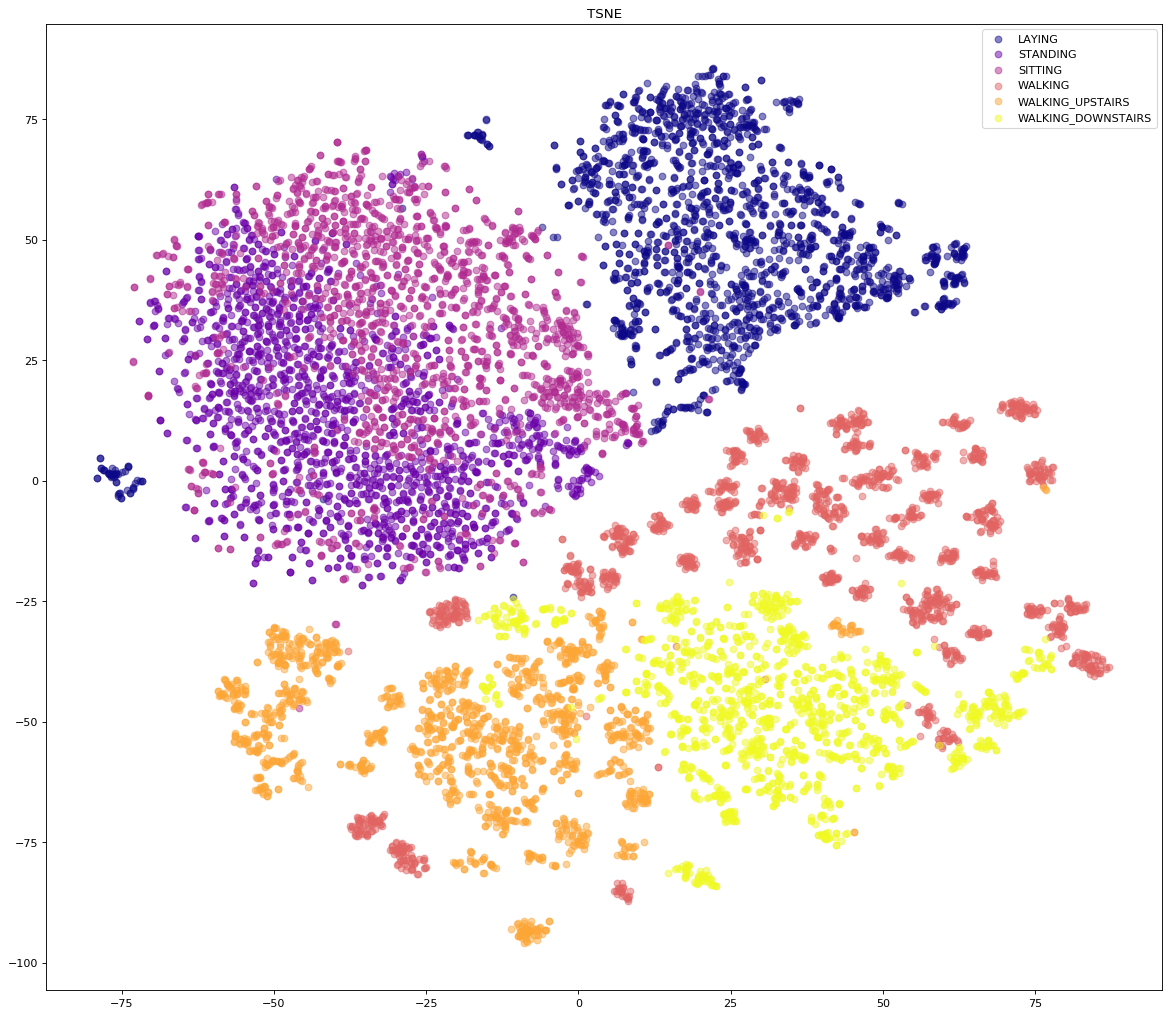
\includegraphics[scale=0.30]{tsne.png}
	\caption{t-SNE visualization}
\end{figure}\noindent
From the figure it appears that somewhat that KNN should work best although it might not work better for class labels \textit{STANDING} and \textit{SITTING}.
\section{Experimental Verification}
I trained the data using the following models on two data sets one with original number of features(561) and the tsne transformed data.
\begin{itemize}
	\item Decision Tree
	\item Random Forest
	\item KNN
	\item SVC
	\item Naive Bayes
\end{itemize}
The following results were obtained for original dataset - \\
	\begin{figure}[H]
			\centering
			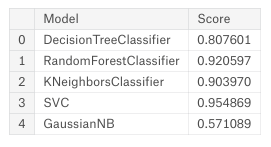
\includegraphics[scale=0.75]{model1.png}
		\end{figure}
\vspace{0.5cm}		
\noindent
The following results were obtained for original dataset - \\
	\begin{figure}[H]
			\centering
			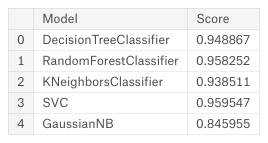
\includegraphics[scale=0.75]{model2.png}
		\end{figure}
\vspace{0.5cm}
Clearly by reducing the dimension we are not losing something. Hence it is better to transform the data two 2 dimensions and then train our model.

My hypothesis that KNN should work better is not clearly visible here as the labels \textit{STANDING} and \textit{SITTING} data points are nearby. Hence it will be better to make a our model by combining the power of different models.

So we will train the whole data using KNN and train the data points with labels \textit{STANDING} and \textit{SITTING} using SVC. Now while predicting our answer we will use KNN, if KNN predicts \textit{STANDING} or \textit{SITTING} then we will use SVC's prediction.
\newpage
\begin{figure}[H]
	\centering
	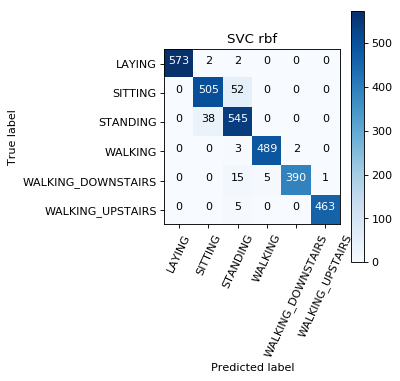
\includegraphics[scale=0.450]{svc.png}
	\caption{Confusion Matrix for SVC rbf}
\end{figure}
\begin{figure}[H]
	\centering
	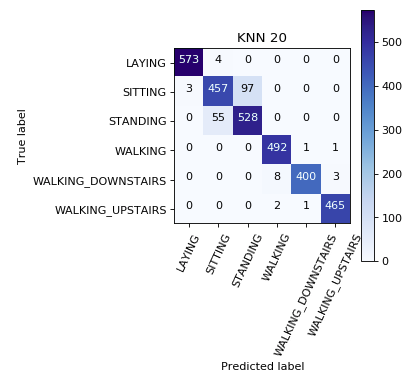
\includegraphics[scale=0.450]{knn.png}
	\caption{Confusion Matrix for KNN K=20}
\end{figure}
\begin{figure}[H]
	\centering
	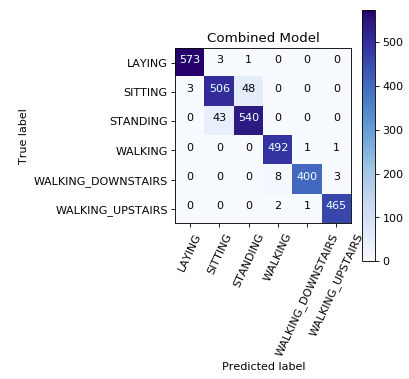
\includegraphics[scale=0.450]{combo.png}
	\caption{Confusion Matrix for Final model}
\end{figure}
By this model we combine the prediction capabilites of both KNN and SVC. Final acuracy is around $\sim$96.5 $\%$.
\begin{figure}[H]
	\centering
	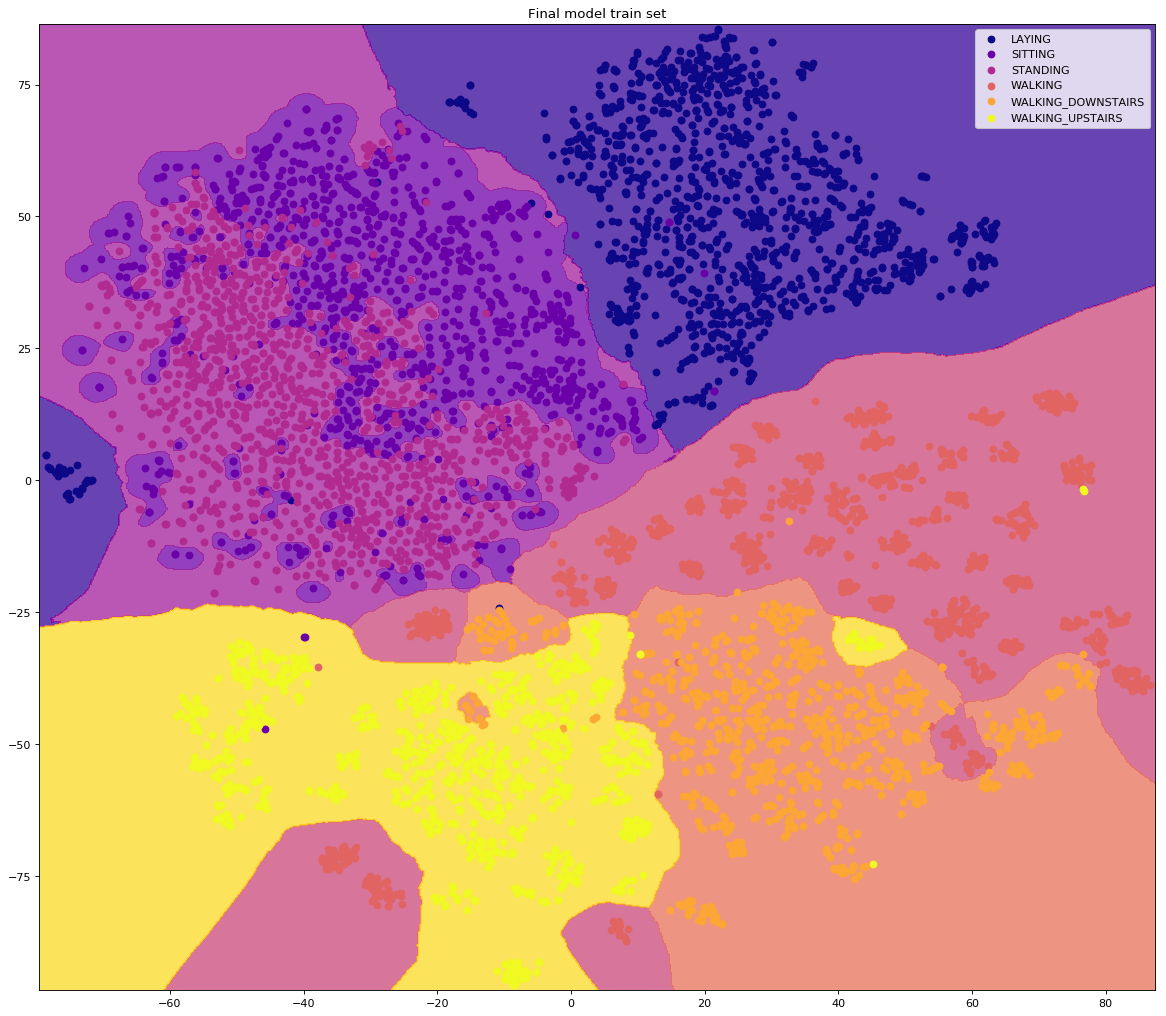
\includegraphics[scale=0.30]{result_train.png}
	\caption{Result on train set}
\end{figure}\noindent
\begin{figure}[H]
	\centering
	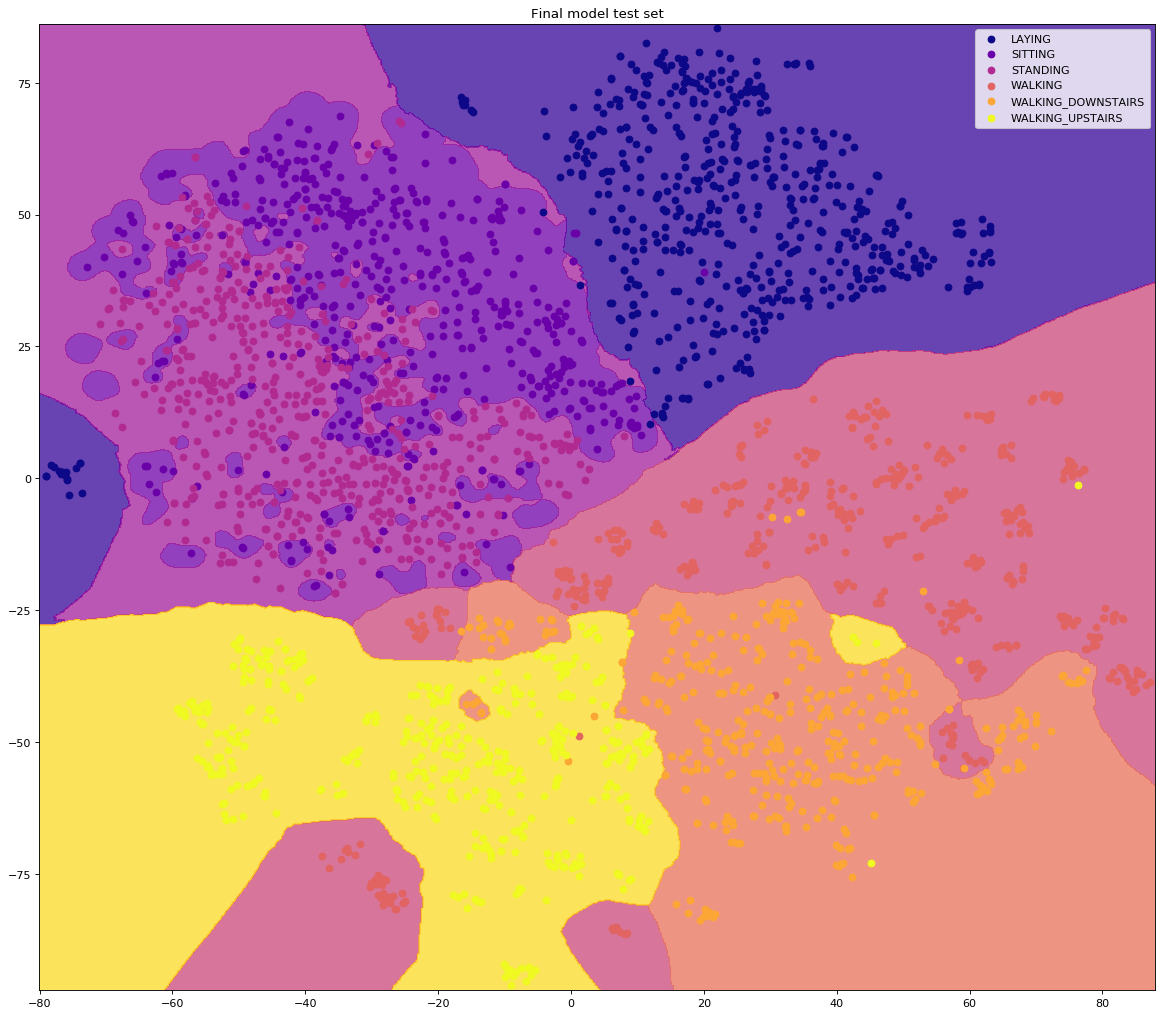
\includegraphics[scale=0.30]{result_test.png}
	\caption{Result on test set}
\end{figure}\noindent
\section{Challenges faced}
\begin{itemize}
	\item \textbf{Chosing the right model} - I was confused between SVC and KNN. SVC was more accurate where as KNN was more intuitive. At last with Ma'am advice I went with a combined model as metioned above.
	\item \textbf{t-SNE vs PCA and other models} - This was a little tricky. As my data set had 561 dimensions, it was not practical to visual it as such. So I used tsne to gain more insights about the data. Later, as tsne was oreserving most of the data I chosed to train my model in 2 Dimensions.
	\item \textbf{Using Kaggle kernels and notebooks} I learned the power of notebooks and the flexibilty that they offer. This project made me familiar with Kaggle interface and their kernels(which are quite powerfull).
\end{itemize}
\section{Links}
	Data Set - \href{https://archive.ics.uci.edu/ml/datasets/Human+Activity+Recognition+Using+Smartphones}{UCI Machine Learning Repository}\\
	Kaggle Kernel - \href{https://www.kaggle.com/nikhilyadv/kernelb8e59d4169}{Nikhil}\\
	GitHub Repository - \href{}{nikhilyadv}
\end{document}